%\documentclass{sig-alternate}
\documentclass[10pt,conference,letterpaper]{IEEEtran}
\usepackage{graphicx}
\usepackage{amsmath}
\usepackage{algorithm}
\usepackage{algorithmic}
\usepackage{graphicx}
\usepackage{epstopdf}
\usepackage{epsfig}
\usepackage{color}
\usepackage{amssymb}
\usepackage{flushend}
\usepackage{stfloats}
\usepackage{subfigure}
\usepackage{url}
\usepackage{verbatim}
\usepackage{lipsum}
\usepackage{multirow}
\usepackage[T1]{fontenc}
\usepackage{mathtools}   % loads »amsmath«

\newtheorem{theorem}{Theorem}
\newtheorem{lemma}[theorem]{Lemma}
\newtheorem{proposition}[theorem]{Proposition}
\newtheorem{corollary}[theorem]{Corollary}

\newenvironment{definition}[1][Definition]{\begin{trivlist}
\item[\hskip \labelsep {\bfseries #1}]}{\end{trivlist}}
\newenvironment{example}[1][Example]{\begin{trivlist}
\item[\hskip \labelsep {\bfseries #1}]}{\end{trivlist}}
\newenvironment{remark}[1][Remark]{\begin{trivlist}
\item[\hskip \labelsep {\bfseries #1}]}{\end{trivlist}}

\newcommand{\listenv}
{\setlength{\itemsep}{0in}\setlength{\parsep}{0in}}

\newcommand{\fig}[1]{Figure~\ref{#1}}
\newcommand{\tab}[1]{Table~\ref{#1}}
\newcommand{\alg}[1]{Algorithm~\ref{#1}}
\newcommand{\property}[1]{Property~\ref{#1}}
\newcommand{\sect}[1]{Section~\ref{#1}}

\newtheorem{defn}{Definition}
\newtheorem{exam}{Example}
\newtheorem{observ}{Observation}
\newtheorem{prop}{Property}
\newtheorem{lema}{Lemma}

\newcommand{\reminder}[1]{{\bf ** #1 **}}
\newcommand{\eat}[1]{}



\begin{document}

\title{Efficient Probabilistic Skyline operator over Uncertain data using Mapreduce}


\maketitle

\begin{abstract}
This paper presents an efficient probabilistic skyline algorithm over uncertain data using mapreduce.
\end{abstract}

\section{Introduction}\label{sec:intro}
Uncertain database management has been studied extensively, and skyline query over uncertain database provides many significant applications, such as multi-criteria decision-making over uncertain data. Given an uncertain dataset containing k-dimensional objects, each object is represented by a weighted set of tuples called instances and follows a discrete probabilistic distribution. Probabilistic skyline computation finds the probability of each object being in the skyline set, or its skyline probability. A number of efficient algorithms~\cite{pei2007}~\cite{atallah2009}~\cite{bohm2009}~\cite{kim2011} have been proposed for Probabilistic skyline evaluation, but they all focus on solving the problem in a single machine.

Besides, when comes to skyline query for large datasets, the straightforward approach is to parallel the skyline processing, which also has drawn a lot of interests recently~\cite{ref:SkylineQueries}~\cite{ref:SkylineMulticore}~\cite{ref:SkylineDistributed}~\cite{ref:RandomPartition}. However, All previous algorithms are concentrated on paralleling the traditional skyline query, not probabilistic skyline query. In this paper, we focus on evaluating the probabilistic skyline query over uncertain database using MapReduce~\cite{ref:MapReduce}. In addition, mapreduce has been incorporated into increasing number of database applications~\cite{ref:KNNMapReduce}~\cite{ref:KNNJoin}~\cite{ref:SetSimilarity}~\cite{ref:ThetaJoins}.

Our work is most related to ~\cite{ding2012}, as they also concentrated on distributed skyline queries over uncertain data. However, Ding et al.~\cite{ding2012} assumes that every tuple in distributed uncertain database is attached with a probability, which could be regraded as a bivariate distribution, rather than multivariate distribution. Obviously the assumption is not in accord with real world. In addition, their algorithm can not be evaluated in mapreduce architecture, and is not efficient.


%\subsection{Motivations}


\section{Preliminaries}\label{sec:prelim}
\subsection{Probabilistic Skyline over Uncertain Data}
Given a d-dimensional data set, skyline query returns a set of points that are not dominated by any other points. A point \(p\) dominating a point \(q\) is denoted as \(p \prec p\); conversely, \(p \nprec p\) represents that \(p\) is not able to dominate \(q\). The domination relationship between points can be easily extended to group relationships easily. For example, \(p \prec D\) denotes that \(p\) dominates all points in \(D\). Next, let us introduce the components of uncertain datasets.

Let \(OS= \{O_{1},O_{2},\dots,O_{n}\}\) denotes the uncertain object set, and the number of objects is \(n\). We assume that an certain object has several instances, each of which is a d-dimensional attribute vector and has a probability to happen. Formally, \(O_{i}\) has an instance set \(O_{i} =\{p_{1},p_{2},\dots,p_{m}\}\), consisting of multiple \(d\)-dimensional instances with discrete probability density distribution of \(O_{i}\). Any instance \(p\)'s occurance probability \(Pr(p)\) only depends on the object's \(pdf\)(probability density distribution), i.e., every object is independent of each other. We assume that \(\sum_{p\in O}Pr(p) = 1\) applies for every object \(O_{i}\). This is a realistic assumption adopted in many literatures~\cite{pei2007}~\cite{bohm2009}~\cite{kim2011} for analyzing uncertain data.

Now we introduce the definition of Probabilistic Skyline, whose definition is quite different from traditional skyline. The goal of Probabilistic Skyline is to obtain the skyline probability \(SKYProb(O_{i})\) of one object \(O_{i}\) in the skyline set, i.e., the likelihood that \(O_{i}\) becomes a skyline point. Given two Objects \(O_{u}\) and \(O_{v}\), the probability that one instance \(p\) in \(O_{v}\) is dominated by another object \(O_{u}\) is:

\begin{equation}
Pr(O_{u} \prec p) = \sum_{q \in O_{u} \; q \prec p}Pr(q)
\end{equation}

Intuitively, the probability that \(p\) is a skyline instance for \(O_{u}\) is equal to that \(p\) is not dominate by \(O_{u}\), which can be represented by:

\begin{equation}
Pr(O_{u} \nprec p) = 1 - \sum_{q \in P_{u} \; q \prec p}Pr(q)
\end{equation}

Then we obtain the probability that \(p\) is not dominated for all objects in \(OS\) except $O_v$, which can be regarded as the likelihood of  $p$ to be a global skyline instance. As objects are independent of each other, \(SKYProb(p)\) (\( p \in O_{v}\)) is computed as follows:

\begin{equation}
SKYProb(p) = \prod_{O_{u} \in OS \; O_{u} \ne O_{v}}(1 - \sum_{q \in O_{u} \; q \prec p}Pr(q))
\end{equation}

Finally, for object \(O_{v}\), we are able to obtain the skyline probability that \(O_{v}\) is a skyline object:
\begin{equation}
\label{equ_final}
SKYProb(O{v}) = \sum_{p \in O_{v}} Pr(p)SKY Prob(p)
\end{equation}

Given a threshold \(t\), we obtain a object set $Or$, where $SKYProb(O_v)$ of every object is larger than $p$. That is,
\begin{equation}
\label{equ_threshold}
PSKY(OS) = \{ o \in OS|SKYProb(o)>t \}
\end{equation}

\subsection{MapReduce framework} %refer FEFEILI's EDBT12 paper
A typical MapReduce framework consists of two user-defined functions: map and reduce. For every record in the input data sets, map function will partition it into a sorted set of intermediate results. The reduce function fetches the data, from individual partition. provided by the map function, Reduce process produces the final output data. The map and reduce function could be fomally defined: \(map(k_{1},v_{1}) \rightarrow list(k_{2}, v_{2}) \) and \(reduce(k_{2},list(v_{2})) \rightarrow list(k_{3}, v_{3}) \).


\section{A Baseline Method}\label{sec:naive}
It can be found that the arduous part of computing probabilistic skyline is obtaining the sum of weights of all instances that dominate a specific instance in Equation 3. Notice, in our assumption, the dataset is too large to fit into one machine's memory; in fact, all data is distributed in disks of all machines in one cluster. The most straightforward solution is partitioning objects in a pair-wise way, computing probabilistic skyline between one pair of objects in Equation 2 and one instance \(p\)'s skyline probability \(SKYProb(p)\) in Equation 3, merging all instances' intermediate results to the final skyline probability in Equation 4. In this section, we apply the idea to a three-phase and a two-phase MapReduce frameworks.


\subsection{Three-phase MapReduce}
In the first phase of three-phase MapReduce, we create pair-wise comparisons between any two objects. At the end of Map phase, every possible pair of two objects is assigned one key. Assume that the number of objects is \(m\), and the number of the whole instances is \(n\). Therefore, the number of pairs is going to be \(C_{m}^{2}\). In the reduce phase, it fetches the object pair with the key (one of \(C_{m}^{2}\)), say the objects are \(P\) and \(Q\), and performs two block nested loop comparisons. We compute the sum of all instances' weights of P which dominate one instance of Q (Equation2). That is, for every q in Q, $Pr( P\nprec q) $ is computed. Reversely, we compute the value of $Pr( Q\nprec p) $for every p in P.  The results from all reducers are written into \(C_{m}^{2}\) HDFS files.

%In the first phase, all instances of one object are replicated in \(m-1\) bucket for a reduce function, and local probability computing is executed between two objects for every instance in \(P\) and \(Q\).

In the second phase, our target is to find the global skyline probability for each instance. So we read the output from the first phase and use the instance ID key as the partitioning key at the end of Map phase. Hence, every reducer will group all object skyline probability for each instance and do an multiplication of them (Equation3). The output from second phase reducers are written into \(n\)(\(n\) is the whole number of instances of all objects) files in HDFS.

Similarly, in the third phase, output generated by the second phase is read by map function and every object ID is assigned as a new partitioning key for reduce phase. In the Reduce function, We sum all instance's global skyline probability for one object (Equation4) as the final result, that is, the final object skyline probability.

\subsection{Two-phase MapReduce}
For the three-phase MapReduce algorithms, in most times, we have many similar operations in the second and third phase, and it suffer from high I/O overhead. It give us the incentive that we create the two-phase MapReduce function which merge the the process of Equation3 and Equation4.

The first phase in Two-phase MapReduce is the same as in the Three-phase MapReduce. It generates \(C_{m}^{2}\) HDFS files, which contain the local skyline results of every pair of objects. In the second phase, These files are read in the map function, and the object ID is assigned as the partitioning key for the reduce phase; then, in the reduce phase, we create a local hash for every instance read: instance ID is the key in hashing, and instance probability array is its value. Then we compute every instance's global skyline probability by multiplication of all values of one specific instance. After that, the object skyline probability is obtained by the sum of the product of every instance's \(Skyprob\) and its own existing \(Prob\).

It is easily found that efficiency in two-phase algorithms is much higher than in three-phase algorithms.
\subsection{Challenge}
However, it has several restrictions for this approach: (1). how to partition objects evenly is hard, since the number of instances might be highly different in various object. In addition, some object might occupy billions of instances, while some other object occupies dozens; (2). besides, we don't know the distribution of instances of one object in advance. If all the instance of one object always appear in the right-corner of coordinate axis, and the object is certain to be a non-skyline object. The optimal approach should be that the object is pruned in the early stage; (3). for every object, we must put every instance into the machine, which is obviously inefficient. the communication cost of putting every instance into one machine is too expensive, especially the IO cost is high. the detailed analysis is in the next paragraph. One improvement is indexing all points before query begins.



\subsection{Experimental Evaluation}
To compare the performance between three-phase, two-phase Hadoop implementations in one cluster and the straightforward implementation on a single machine, we implemented the three algorithms and conducted a experimental evaluation.

There're several observations found in the experiment:


1). Let me first introduce the result of single-machine algorithm. With increasing size of the dataset, the computing time is increasing exponentially. And the most arduous part in the whole computing procedure is in Equation2.

In the first experiment set, we randomly generated 100 objects, and 1 thousand instances per object. The whole computing procedure for Equation2 involves computing the local skyline probability between any pair of two objects. That is 215.6 seconds in our result. In addition, it needs 0.2s for Equation3 process and 0.02s for Equation4 process. Therefore, the whole running time is less than 216s. It can be found that 99\% of the time lies on Equation2. However, in our hadoop implementation, the whole query time is about 15 mins. Therefore, if the dataset is small, the time consumed in Hadoop is less than one in single-machine algorithm.

In the second experiment set, we randomly generated 100 objects, and 10 thousand instances per object. The test shows that it needs 5 seconds to run Equation2 for every pair of objects. Since we have \(C_{100}^{2}\) pairs, and the time in all is estimated to be more than 7 hours. However, the time consumed in the hadoop implementation is about 4 hours.

2). When compared between two Hadoop implementations, the two-phase Mapreduce framework is always faster than three-phase one. The reason is that the amount of computing is little in the third phase of the three-phase framework, and merging the second and third phase into one phase reduces one copy of reading data from the HDFS to memory, increasing I/O efficiency.

%
%\section{Prob Skyline using MapReduce}\label{sec:design}
%In this section, we propose our design of probabilistic skyline evaluation using kd-tree upon MapReduce environment.

The general idea is that we evenly split the whole instances to several subsets put into several machines, and let every machine compute the equation 3 of every instance. After instances' probabilistic skyline results are obtained, the intermediate results are merged in a machine to compute the final object probabilistic skyline answer through Equation 4.

There are three major considerations that affect the performance of computation.

\begin{enumerate}
  \item The cost suffered from Shuffling data from Map to Reduce.
  \item The cost of figuring out the Pskyline answer of all instances in the reduce phase.
  \item The cost of merging all intermediate results to answer final object Pskyline value.
\end{enumerate}

\subsection{Paralleling using kd-Tree}
our task is to build a balanced k-d tree~\cite{kd} of N points to m machines. For simplicity and convenience of presentation, N and m are assumed to be powers of two. Before presenting the construction of distributed kd-tree, we introduce the definition of a k-d tree.

Consider a set of k-dimensional points. A k-d tree is a binary tree upon the points. The root of it is the original set of points, and the subtrees are root's children. The construction of k-d tree starts with choosing one of the k dimensions, finding the median of the points. The median along the dimension generates a splitting hyperplane that divides the set of points into two equal sized sets. The two sets are put into the left and right subtree (child) of the root respectively. The construction recursively generates the subtrees by finding the new medians of two subsets along another dimension, splitting the hyperplane along the dimension, until each leaf corresponds to only one point.

We are able to observe that the number of points in every subtree upon the same level is (approximately) the same, since the parent always generates children by splitting median. It gives us the incentive to compute instances' probabilistic skyline results using MapReduce.

Recall that we have m machines and m is powers of two. We partially constructed k-d tree in which nodes and leaves are within $log$\hspace{0.03 in}$m$ levels. Let the preprocessing step launch a master node to construct k-d tree within $log$\hspace{0.03 in}$m$ levels. A small variation is made for the k-d tree: points are only stored in leaves. Nodes other than leaves are only a hyper-rectangle. After that, every leaf in the k-d tree is composed of N/m points, and bounded by a k-dimensional hyper-rectangle. The frontiers of the rectangle is delimited, and is going to be one key in the Map phase later. We store the frontier information of m leaves into DFS (Distributed File System).
%The modification can be designed by sliding split hyperplane from original place to guarantee no points is cut-off by splitting~\cite{maneewongvatana1999s}.


Then a MapReduce job is launched to map all the points to m slave machines and collect statistics of each object. Before the Map phase is launched, the frontier information is loaded to memory from DFS in each mapper. The mapper reads instances, justifies what split the instance is belonged to, assigns one split key for the instance.

In addition, the map phase aggregates statistics of every object. An in-memory table is created and maintained for statistics. It can be implemented by well-known distributed shared memory~\cite{DSM} easily. Assume $|O|$ is the number of objects. The table collects the object ID, the minimum coordinates, the maximum coordinates. It is easily collected since mappers read all instances, and is able to obtain the maximum and minimum value by only comparing its current coordinate with the value in the table.
The maximum and minimum coordinates of every object benefit query process by pruning some objects that don't need to be considered.

\subsection{Reduce Phase}
After map phase, all instances are mapped to designated reducers, and ready to perform probabilistic skyline. The Reduce Phase is launched with constructing uncompleted k-d tree from the current root, which is the rectangle bounded by its frontiers passed. The kd-tree construction continues until each leaf corresponds to one point.

For any node rather than leaf, represents a hyper-rectangle bounded for its children, all of which are within the rectangle. For a node $R$, in the following Skyline computation, instances other than those in R are looked up to find the domination relationship with $R$. For an instance \(p\) outside $R$, there exist three scenarios of relationships: $R$ is dominated by $p$ (all instances in $R$ are dominated by $p$); some area of $R$ is dominated by some instance (The domination area of $R$ intersects one of $p$); some instance is fully dominated by R (All instances in $R$ dominate $p$).

After the tree is constructed, we pre-order traversal

%
\section{MapReduce Framework}\label{sec:mapreduce}
To overcome the above challenges, we propose the two-phase MapReduce algorithms \textit{MP-ProbSky}, as shown in Figure~\ref{figure:framework}. $MP-ProbSky$ contains two main MapReduce phase. In the first phase, it contains two procedures:

(1) \textbf{filtering unqualified objects:} After instances of objects are mapped to $N$ reducers through angle-based partition scheme, unqualified objects are filtered out based on three pruning rules, as these unqualified objects are not able to be in the $p-$skyline object set. 

(2) \textbf{collecting data:}
Objects which are not filtered in this phase become candidate objects. In addition, instances dominating candidate objects are collected since they are important to collecting the actual skyline probability. The two varieties of data are outputted in the reduce function. 

In the second phase(See Section~\ref{sec:second}), all candidate objects are grouped into several machines based on a novel grid partition, and object skyline probability is computed locally in separate machine. After that, $p-$skyline object set is easily obtained.
\begin{figure*}[t]
\centering
  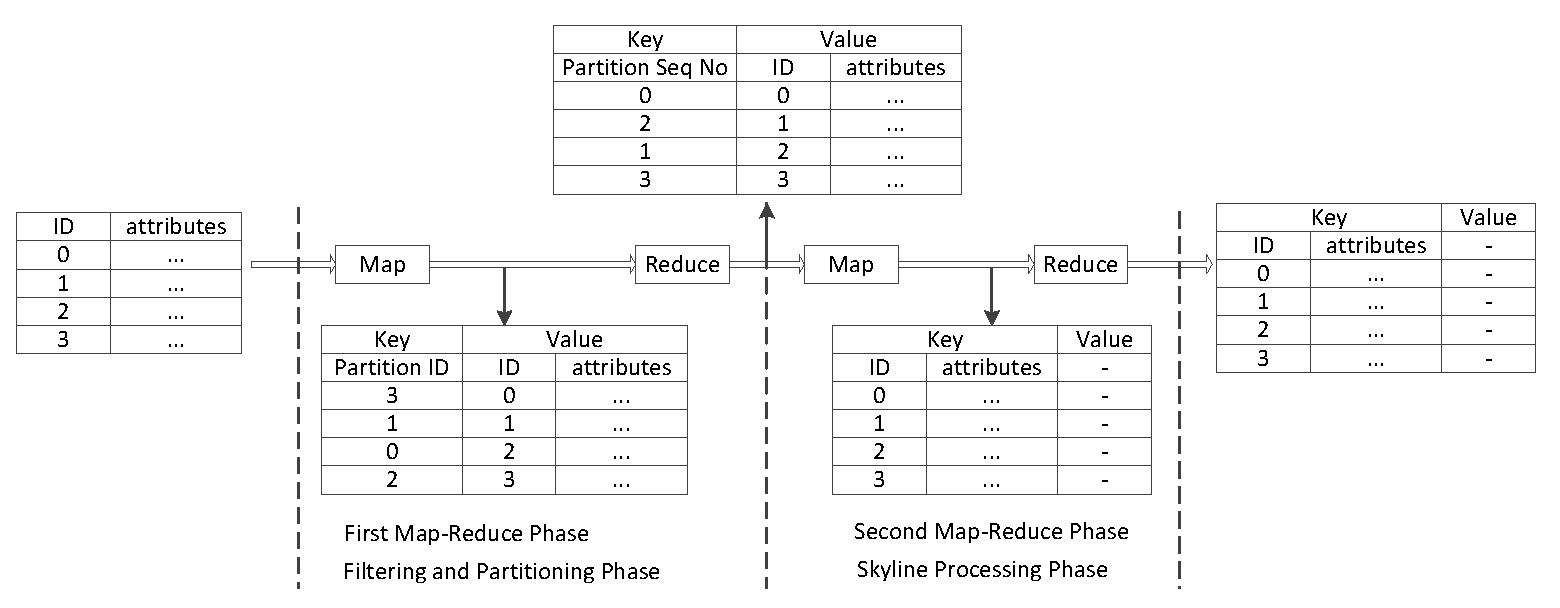
\includegraphics[width=0.9\textwidth]{figs/framework.eps}
  \vspace*{-10pt}
  \caption{An overview of parallel skyline processing using MapReduce.}
  \vspace*{-15pt}
  \label{figure:framework}
\end{figure*}

\subsection{Partitioning}

Angle-based space partitioning scheme~\cite{ref:AngularPartition} transforms data point from Cartesian coordinate to hyperspherical coordinate. In the first map phase, we use angle-based partitioning strategy to map data points into N partitions. The main advantage of angular transformation is that this strategy being able to filter data points as much as it can since the left bottom corner data points dominate most other data points in an angle.

Given a d-dimensional data point $p = [p_1, p_2, \dots, p_d]$, the hyperspherical coordinates of $p$ include a radial coordinate $r$ and $d-1$ angular coordinates $\varphi_1, \varphi_2, \dots, \varphi_{d-1}$~\cite{ref:AngularPartition}, denoted by $\{r, \varphi_1, \varphi_2, \dots, \varphi_{d-1}\}$, where r is the distance to the origin, and $\varphi_i$ represents an angular coordinate $ 0 \leq  \varphi_i \leq \frac{\pi}{2}$. Similarly, an angle-based space partition is represented by $V^A = \{\Phi_1^A, \Phi_2^A, \dots, \Phi_{d-1}^A \}$, where $\Phi_i^A$ is an angle range $[\varphi_i^j,\varphi_i^k]$ in the $i^{th}$ dimension.

In term with the detailed implementation of the Map Phase, the number of reducers have been defined prior to the launch of the application, and the default partitioning angles $V^A$ has been computed. The whole instance dataset is an input to Map function. 

% In the Map phase, angular coordinates of data point of every instance are computed, and mapped to target reducer.

\subsection{Pruning Power}
Given an object $O = \{p_1, p_2, \dots, p_m\}$, the minimum corner of one object $O_{min}$, is represented by a $d-$dimensional virtual point $( \min\limits_{p_i \in O}p_i[1], \min\limits_{p_i \in O}p_i[2], \dots, \min\limits_{p_i \in O}p_i[d])$, where $p_i$ is an instance in $O$. Similarly, $O_{max}$ is a maximum corner point.

\vspace{5 mm}
\begin{lemma}
\label{lemma:1}
Given $O^a, O^b \in O$, \emph{if} $O^a_{max} \prec O^b_{min}$, then $SKYProb(O^b) = 0$, $O^b \notin PSKY(OS)$.
\end{lemma}

\vspace{5 mm}

\begin{lemma}
\label{lemma:2}
Given $O^a \in O$, an instance $p \notin O^a$, \emph{if} $O^a_{max} \prec p$, $SKYProb(p) = 0$.
\end{lemma}

\vspace{5 mm}

The proof of Lemma~\ref{lemma:1} and Lemma~\ref{lemma:2} is obvious and omitted.
Besides, we compute the probability of one object $O_a$ being a skyline object with partially seen data. And the upper bound of it is denoted by $SKYProb^{+}(O)$. Similarly, $SKYProb^{+}(p)$ represents the probability of an instance $p$ being a skyline instance.

\vspace{5 mm}

\begin{lemma}
\label{lemma:3}
Given $O^a \in O$, $O^a=\{p_1, p_2, \dots, p_m\}$, $|O^a| = m$, $O^a$'s instances are mapped into several partitions (machines). Assume partition $V^A$ has $n$ instances out of $m$ ($n<=m$) for $O_a$, containing instances $\{p_1, p_2, \dots, p_n\}$. Then:

\begin{equation}
\label{objectUpper}
    \begin{aligned}
PrSKY^{+}(O_a) = 1 - \sum\limits_{i=1}^n Pr(p_i)(SKYProb^+(p_i)-1)
    \end{aligned}
\end{equation}

\emph{if} $SKYProb^{+}(O_a) < p$, then $O_a \notin PSKY(OS)$.

\end{lemma}

\begin{proof}
The Skyline Probability of an object $O_a$ is denoted as:
\begin{equation}
    \begin{aligned}
SKYProb(O_a) = \sum\limits_{i=1}^n Pr(p_i)(SKYProb(p_i))
    \end{aligned}
\end{equation}

\begin{equation}
    \begin{aligned}
\sum\limits_{i=1}^n Pr(p_i) = 1
    \end{aligned}
\end{equation}

Then, 
\begin{equation}
    \begin{aligned}
& SKYProb^{+}(O_a) \\
& <= \sum\limits_{i=1}^n Pr(p_i)(SKYProb(p_i)) +
\sum\limits_{i=n+1}^m Pr(p_i) \\
& <= \sum\limits_{i=1}^n Pr(p_i)(SKYProb^+(p_i)) +
1 - \sum\limits_{i=1}^n Pr(p_i) \\
& = 1 - \sum\limits_{i=1}^n Pr(p_i)(SKYProb^+(p_i)-1)
    \end{aligned}
\end{equation}
\end{proof}


\subsection{First Phase}
\label{firstPhase}
Before the first phase MapReduce job is launched, every object $O$'s $O_{min}$ and $O_{max}$ is computed locally by iterating all objects and computing $O_{min}$ and $O_{max}$ of every object.

The first map phase maps data points (instances) to $N$ machines based on angular partition scheme. The defined map function computes every instance's hyperspherical coordinate, and maps instances to designated reducer (machine). In addition, if any instance of one object $O$ is mapped to a reducer $V^A$, maximum and minimum corner of $O$ ($O_{min}$ and $O_{max}$) is also transmitted to the partition. Therefore, $O_{min}$ and $O_{max}$ of one object might appear in more than one partitions, since instances of one object are distributed in more than one partitions.

During the reduce phase, only data in this partition (data in $V^A$) is visible. Objects are firstly examined if some of them is able to be pruned under the Pruning rule 1. The procedure to examine Pruning rule 1 works as follows. A list $L_{min}$ contains all $O_{min}$ of all objects in this partition; similarly, a list $L_{max}$ contains all $O_{max}$ in this partition. Sort-filter-skyline~\cite{icde/ChomickiGGL03} method is an approach to speed up traditional skyline query by presorting instances. Using $SFS$~\cite{ref:SkylineSFS}, data points with the sum of all the dimensions of each point is presorted in ascending. The starting element is retrieved from $L_{max}$, and compared with the elements in $L_{min}$ to check the dominance relationship. Any object whose $O_{min}$ is dominated by any $O_{max}$ in $L_{max}$ is pruned, since it can not be in the $p-$skyline set.

After this, Pruning rule 2 works as follows. In every reducer, we collected remained objects which are not pruned in $L_{min}$. For every instance in these remained objects, we check if an instance $p$ is dominated by some objects's $O_{max}$. If the dominance relationship occurs ($O_{max} \prec p$), $SKYProb(p)$ is marked to $0$ for the instance and it denotes that $p$ can not become skyline instance.

\subsection{Rectangle Pruning}
In this subsection, we propose a novel strategy to apply Lemma~\ref{lemma:3} to filter unqualified objects in partition $V^A$. As we see in Equation~\ref{objectUpper}, before $SKYProb^{+}(O_a)$ is computed, every instance's $SKYProb^{+}(p)$ contained in this partition is computed. Therefore, the challenge comes from how to efficiently collect the probability of every instance $p$ being a skyline instance.
The straightforward method of computing $SKYProb^{+}(p)$ is to iterate every instance in this partition, and compare the dominance relationship between $p$ and every other local instances in this partition. The computing complexity is obviously high as $O(n^2)$.

\begin{figure*}[t]
\vspace*{-20pt}
  \centering
  \subfigure[\vspace*{-5pt} Example.]{
    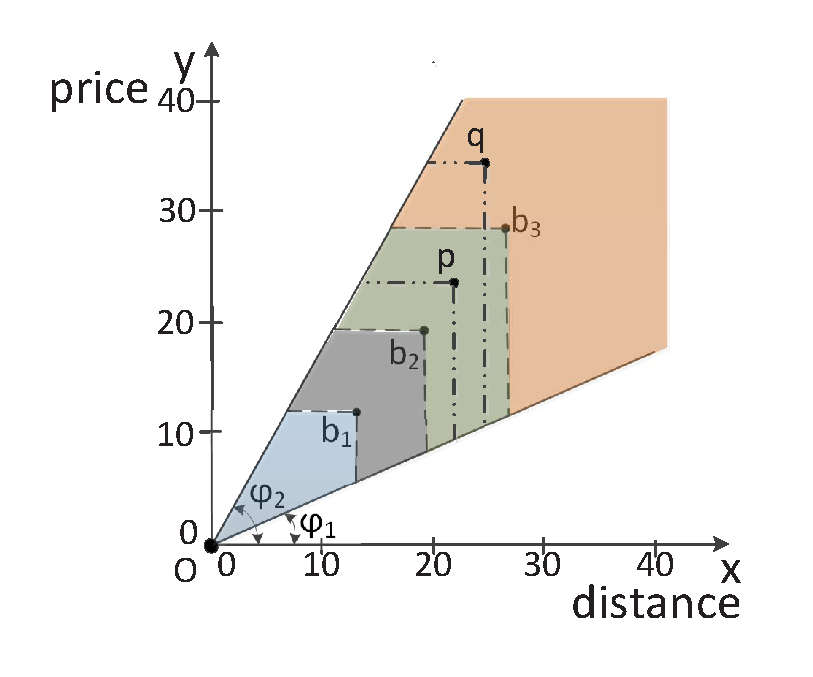
\includegraphics[width=2.3in, height = 4.5cm]{figs/rectExample.eps}}
    \hspace*{-14pt}
  \subfigure[\vspace*{-25pt} Pruning Power Formula.]{
    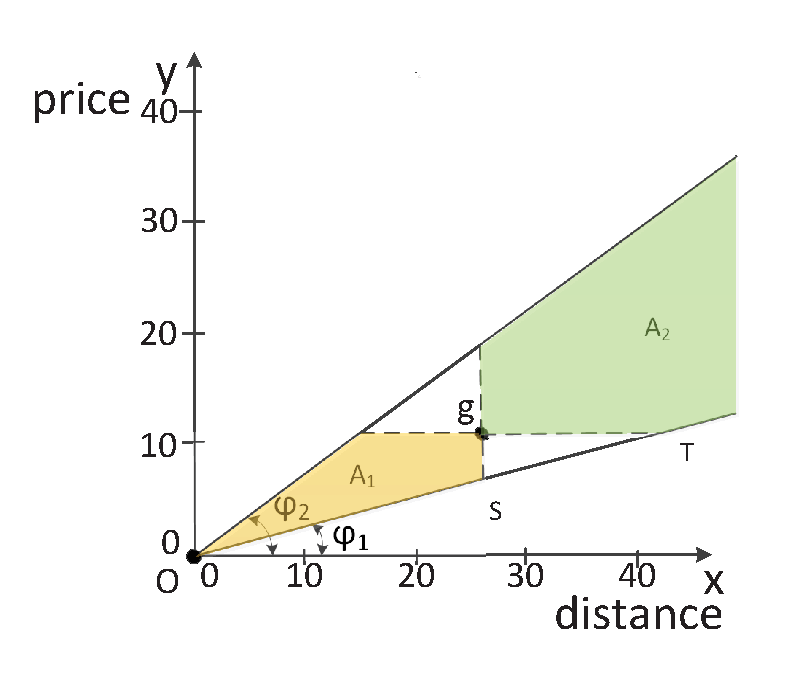
\includegraphics[width=2.3in, height = 4.5cm]{figs/computeA_1.eps}}
  \subfigure[\vspace*{-25pt} Another example.]{
    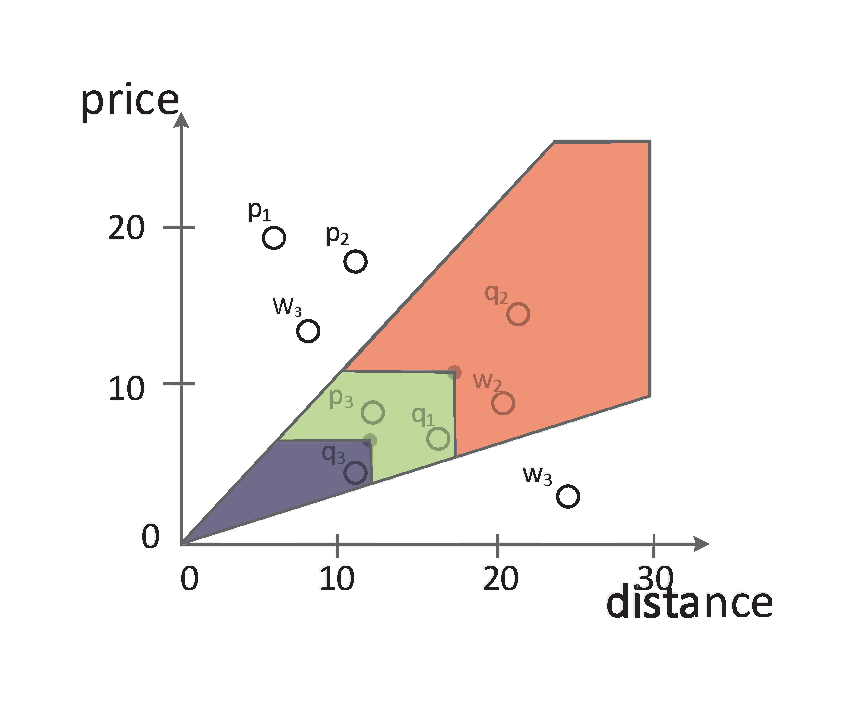
\includegraphics[width=2.3in, height = 4.5cm]{figs/example_phase1.eps}}
  \label{figure:rect}
    \caption{Pruning Power.}
\vspace*{-16pt}
\end{figure*}


One interesting observation is that data points close to maximum boundary are often dominated by data points close to minimum boundary. The intuitive idea is to associate data points close together into a group. Pre-computing is done in the group before probabilistic skyline process is launched. Data points fully dominated by the group is able to speed up processing by repeatedly applying the pre-computed information.


\begin{algorithm}[htp]
  \SetKwFunction{algoMap}{map}
  \SetKwFunction{algoReduce}{Reduce}

  \SetKwInOut{Input}{input}
  \SetKwProg{map}{Algorithm}{}{}
  \map{\algoMap{}}{
  \KwIn{object set $OS$, angle partition array $a$}
  \BlankLine 

	\ForEach{object $u \in OS$ }{
	  \ForEach{instance $p \in u$ }{
	    \tcc{$S^3$ Decide the angle partition which have $p$}
	    $a_{j} \leftarrow S^3(p)$ \;
	    output(j, (p, MIN(u), MAX(u)) ) \;
	  }
	}
  }{}
    \BlankLine 
    \BlankLine 

  \setcounter{AlgoLine}{0}
  \SetKwProg{reduce}{Algorithm}{}{}
  \reduce{\algoReduce{}}{
  \KwIn{instance Array $Arr_i$, object Maximum and Minimum corner point Array $Arr_{max}$, $Arr_{min}$, }
  \BlankLine 

  $O_c \leftarrow \emptyset$ \;
  $I_n \leftarrow \emptyset$ \;

  \tcc{Pruning Rule 1}
  \ForEach{object $u \in Arr_{min}$ }{
  	$O_c \leftarrow u$ \;
  	\ForEach{object $v \in Arr_{max}$ $\&\&$ $v \prec u$}{
  		$O_c.remove(u)$ \;
  		break \;
  	}
  }
  \tcc{Pruning Rule 2}
  \ForEach{object $u \in O_c$ }{
  	\ForEach{instance $p \in u$}{
	  	\ForEach{object $v \in Arr_{max}$ $\&\&$ $v \prec u$}{
	  		$I_n \leftarrow p$ \;
	  		break \;
	  	}
  	}
  }
  \tcc{Pruning Rule 3}
  \Return Rectangle Pruning($O_c$, $I_n$) \;
  }
  \caption{First Phase Procedure}
\end{algorithm}


\begin{algorithm}[!t]
\label{RectanvlePruning} 
\SetKwInOut{Input}{input}
\SetKwInOut{Output}{output} 
\caption{Rectangle Pruning}

\KwIn{object set $OS$, instance set $I_s$} 
\KwOut{candidate object $O_c$, influence instance set $I_p$}

\BlankLine 

\Return $O_c$;

\end{algorithm}


Take 2-dimensional data as an example (See Figure~\ref{figure:rect}). Assume the angle of partition $V^A$ is between $\phi_1$ and $\phi_2$. Three virtual data points $b_1$, $b_2$ and $b_3$ separate $V^A$ into four areas, denoted by 4 colors, blue, grey, green and red in order. Every point stands at the maximum corner of a bounding box. $p$ is an instance located in green area. It is observed that $p$ is always dominated by any instance in blue and grey areas since $b_2$ dominates $p$, and $p$ is also affected by partial instances in green area. Similarly, all instances in blue and grey areas and partial instances in green and red areas dominate $q$. According to this observation, we are able to precompute the sum of existing instance probabilities in blue and grey areas, and use the intermediate result for computing $SKYProb^{+}(p)$ and $SKYProb^{+}(q)$. Obviously it is able to speed up the skyline probability computing. 

We use pivot point set $P$ to represent the virtual data points (in Figure~\ref{figure:rect}(a)), defined as a set of d-dimensional data points whose cardinality is m, $P=\{b_1, b_2, \dots, b_m\}$. $A_i$ is denoted as the d-dimensional hyper-rectangle, the minimum corner of which is the origin, and the maximum corner of which is $b_i$. If some point is dominated by $b_i$, it is dominated by any instance in $A_i$. Formally let each area $A_i$ consists of an n-dimensional vector $V_i = [p_{r1}, p_{r2}, \dots, p_{rn}]$, where $n$ is the number of objects in this partition (reducer), and each element $p_{ri}$ is the sum of instance probability for object $O_i$. These vectors is able to repeatedly contribute to the skyline probability of data points.  



Now the problem turns to studying the pruning power of a pivot point $g$. We make the assumption that our dataset is defined in the hypercube $[0,1]^d$ and data points are uniformly distributed. Followed by this assumption, the number of data points located in a region could be represented by the region's volume. To simplify the model of pruning power, only one pivot point exists and it divides the angle area into two parts denoted as $A_1$ and $A_2$. $A_1$ lies in the left bottom to g, and $A_2$ lies in the right top to g. Figure~\ref{figure:rect}(b) depicts the scenario. The pruning power could be represented by how many data points in $A_2$ is able to repeatedly use $A_1$ directly without comparing one by one, since intermediate sum of instance probability in $A_1$ has been computed well. Therefore, given a pivot point $g$, the pruning power of $g$ is defined as:

\begin{equation}
PP(g) = A_1(x_g, y_g, \phi_1, \phi_2) * A_2(x_g, y_g, \phi_1, \phi_2)
\end{equation}
where $A_1$ or $A_2$ is a function, which computes corresponding area shown in Figure~\ref{figure:rect}(b).

In~\cite{ref:AngularPartition}, how to compute $A_2$ is introduced. Three cases are considered in formula induction: one is $0 \leq \phi_1 < \phi_2 \leq \pi/4$, the other is $\pi/4 \leq \phi_1 < \phi_2 \leq \pi/2$, and the final one is $0 \leq \phi_1 \leq \pi/4 \le \phi_2 \leq \pi/2$. The detailed formula is shown in Equation~\ref{Equ:A2}.

\begin{equation}
\label{Equ:A2}
A_2 = 
\begin{cases}
& \int_{x_g}^{1} \int_{x tan \phi_1}^{x tan \phi_2} dydx- \int_{x_g}^{min(1, \frac{y_g}{tan \phi_1})} \int_{x tan \phi_1}^{y_g} dydx  \\
& \qquad \qquad \qquad \qquad \mbox{if } 0 \leq \phi_1 < \phi_2 \leq \pi/4 \\ 
& A_2(g_y, g_x, \frac{\pi}{2} - \phi_2, \frac{\pi}{2} - \phi_1)\\
& \qquad \qquad \qquad \qquad \mbox{if } \pi/4 \leq \phi_1 < \phi_2 \leq \pi/2 \\
& A_2(x_g, y_g, \phi_1, \frac{\pi}{4}) + A_2(g_y, g_x, \frac{\pi}{2} - \phi_2, \frac{\pi}{4}) \\
& \qquad \qquad \qquad \qquad \mbox{if } 0 \leq \phi_1 \leq \pi/4 \le \phi_2 \leq \pi/2
\end{cases}
\end{equation}

Similarly, we compute the area of $A_1$, which is the region defined by $0 \le x \le x_g$, and $x tan(\phi_1) \le y \le min(x tan(\phi_2), y_g)$. Therefore, $A_1$ is represented by 

\begin{equation}
A_1 = \int_{0}^{x_g} \int_{x tan(\phi_1)}^{ min(x tan(\phi_2), y_g) } dydx
\end{equation}


Assume that $0 \leq \phi_1 < \phi_2 \leq \pi/4$, $PP(g)$ is represented by 
\begin{equation}
\begin{aligned}
PP(g) = & (\int_{x_g}^{1} \int_{x tan \phi_1}^{x tan \phi_2} dydx- \int_{x_g}^{min(1, \frac{y_g}{tan \phi_1})} \int_{x tan \phi_1}^{y_g} dydx)  \\
  & * \int_{0}^{x_g} \int_{x tan(\phi_1)}^{ min(x tan(\phi_2), y_g) } dydx
\end{aligned}
\end{equation}

It is found that the pruning power is dependent on the cardinality of $P$ and the placement of $P$ in the partition. Given the formula of pruning power computation, the set of pivot points is studied via experiment. We assume the 2-dimensional space is partitioned into 4 partitions. In each angle partition, the same experiment is executed.


We firstly study the relationship between the number of pivot points and the pruning power. We iteratively sample N points, from 1 to 100. For every iteration, pivot points are sampled 10,000 times. We obtain the pruning power of every iteration based on the sum of all 10,000 samples' pruning power value. For example, when $N=3$, three nodes are uniformly sampled in one partition. the sum of pruning powers of the three points is repeated 10,000 times and the addition of all is the final result. The experiment results shows that the pruning power increases with the elevation of the number of pivot points. Secondly, the distribution of pivot points is studied. We assume that only 1 pivot point is put in the partition. After sampling 10,000 times, we are looking for the location of pivot point, which has the most pruning power. Figure~\ref{figure:PP}(b) shows the experiment results at angle range of $[\pi/8, \pi/4]$. The more powerful pruning power area looks darker red. The pivot points in $( 0.4 \leq x \leq 0.6, 0.4 \leq y \leq 0.6)$ area have the most powerful pruning power.


\begin{figure*}[t]
\vspace*{-20pt}
  \centering
  \subfigure[\vspace*{-5pt} Num Pivot Point.]{
    \label{anchor}
    \includegraphics[width=2.3in, height = 4.5cm]{Exper/NumPruningPower/numPruning.eps}}
    \hspace*{-14pt}
  \subfigure[\vspace*{-5pt} Pruning Power.]{
    \label{watchtower}
    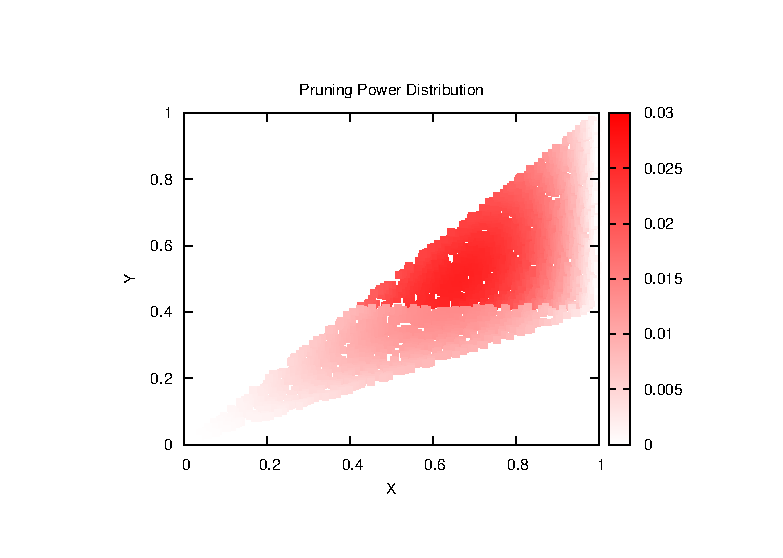
\includegraphics[width=2.3in, height = 4.5cm]{Exper/MostPruningPower/3d.eps}}
    \hspace*{-14pt}
  \subfigure[\vspace*{-5pt} Pivot Points placement.]{
    \label{watchtower}
    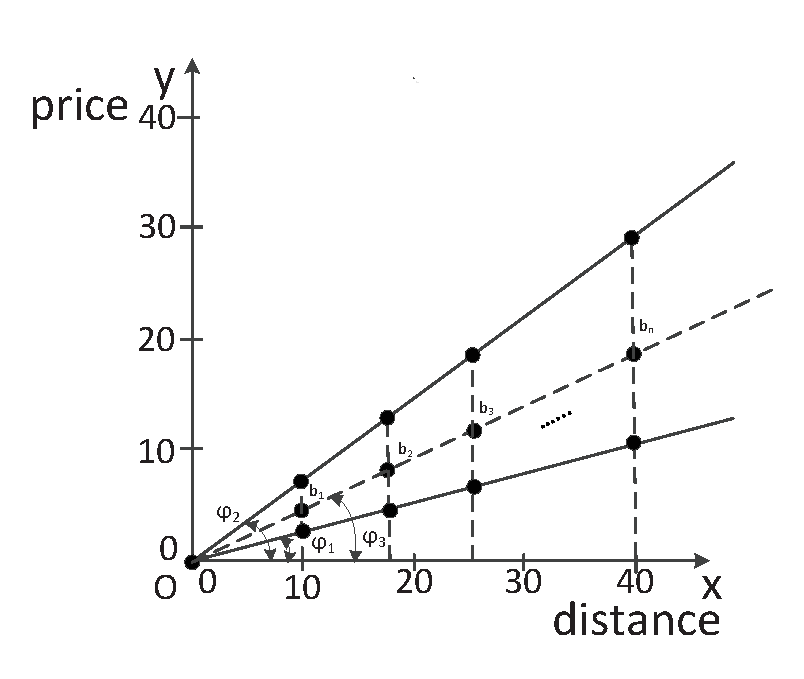
\includegraphics[width=2.3in, height = 4.5cm]{figs/midLine.eps}}
\vspace*{-5pt}
  \caption{Pruning Power.}
  \label{figure:PP}
\vspace*{-16pt}
\end{figure*}

Given the number of pivot points, we propose an efficient strategy to utilize the pruning power of pivot points. Pivot points in $P$ are selected every even interval of x, and are lied in a line $L$ at an angle of $\phi_3$ ($ \phi_2 < \phi_3 < \phi_1 $) (See Figure~\ref{figure:PP}(b)).
Given pivot point set $P$ is placed well, the detailed computing procedure is as follows. Remember $A_i$ consists of an n-dimensional vector $V_i = [p_{r1},p_{r2},\dots,p_{rn}]$, where n is the number of objects in this partition. $V_i$ is maintained in the first step. At the beginning of the reduce phase, the local machine knows which objects are in this partition. Given an instance $p$ of object $O_q$, we firstly search the nearest pivot point $b_i$ dominated by $p$. Then the instance probability is added to $p_{rq}$ in $V_i$. We iterate every instance in the partition and maintain $V_i$ ($ 1 \leq i \leq n$). 

After $V_i$ is finished maintaining, every instance $p$ is iterated for computing $SkyProb^+(p)$. Assume an instance $p$ lies in the area $A_m$. we looks for the nearest $b_i$ which dominates $p$. That is, $A_i$ fully dominates $p$. In addition, we look for area set $S_A$ which partially dominates $p$. $S_A$ = $\{A_j| i < j \leq m \}$.
An additional vector $[p_{r1},p_{r2},\dots,p_{rn}]$ is maintained for comparing domination relationship in $S_A$. If any instance in $S_A$ dominate $p$, the instance's existing probability is counted to the object vector. Then, aggregated by the vectors $V_j$ ($j \leq i$) precomputed already, the product of every element in the object vector is the final $SkyProb^+(p)$.

Then skyline likelihood of every object in $V^A$ is able to be easily obtained by Equation~\ref{objectUpper}. We could prune those unqualified objects with $SKYProb(O)$ less than $p$, and keep remained ones in an object set $C_o$.

\begin{defn}
\label{defn:canObj}
In partition $V^A$, $C_o$ is an object set $C_o = \{ o \in C_o | SKYProb(o) \geq p\}$
\end{defn}

\begin{defn}
\label{defn:influnceInst}
In partition $V^A$, $I_p$ is an instance set $I = \{p \in I_p | \exists p_o \in C_o,  \forall p \prec p_o\}$
\end{defn}

Definition~\ref{defn:canObj} and ~\ref{defn:influnceInst} give the definition of $C_o$ and $I$. After the first MapReduce phase, there are two types of instances remained in $V^A$. In the first case, the instance is belonged to some object in $C_o$ and it is also in $I$. In the second case, the instance is only within $I$. As soon as the data is collected, it is able to move forward to the merging phase.


\section{Second MapReduce Framework}\label{sec:second}
After the first MapReduce phase is completed, the skyline candidate object set $O_c$ is collected. In the next step, the final skyline probability is needed to be computed for determining $p-$skyline object set. In the first MapReduce phase, the angle-based processing only knows the local data at a fixed angle region, and objects remained after pruning decide the final step of merging. Before illustrating our merging algorithm for computing skyline probability, we study the distribution shape of remained candidate objects after the first MapReduce phase.
\subsection{Shape Analysis}

\begin{figure*}[!t]
    \begin{center}
    \vspace{-1.5pc}
  \subfigbottomskip = 2pt \subfigure[Independent Distribution]
    {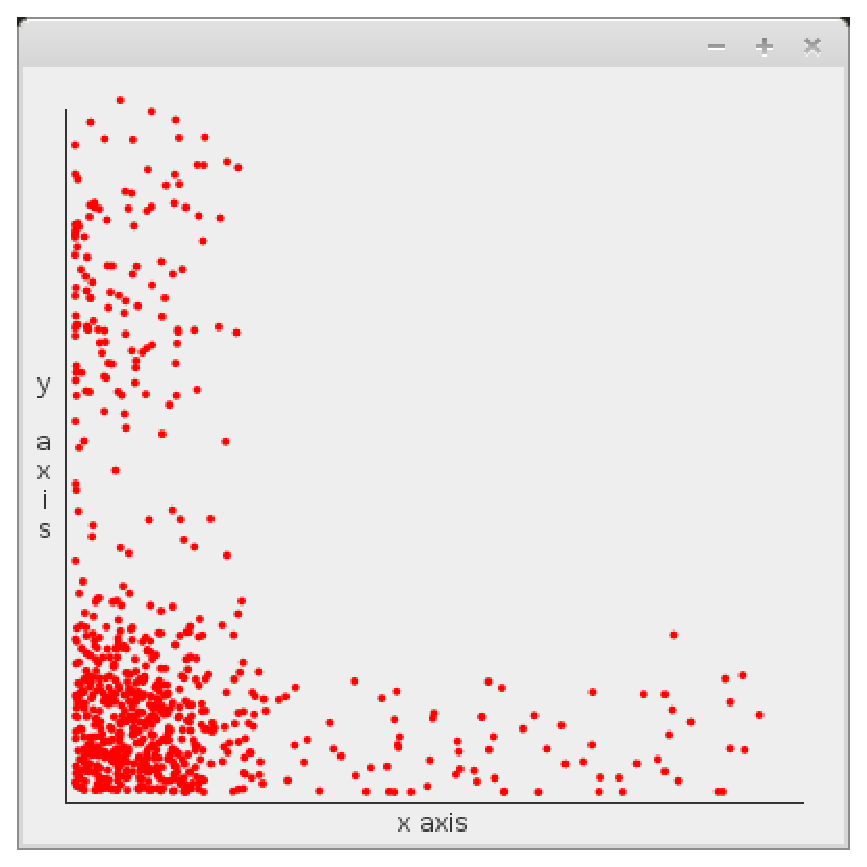
\includegraphics[width=0.24\textwidth]{figs/inde.eps}}
    \hspace{0.01em}
  \subfigbottomskip = 2pt  \subfigure[Anti-correlated Distribution]
    {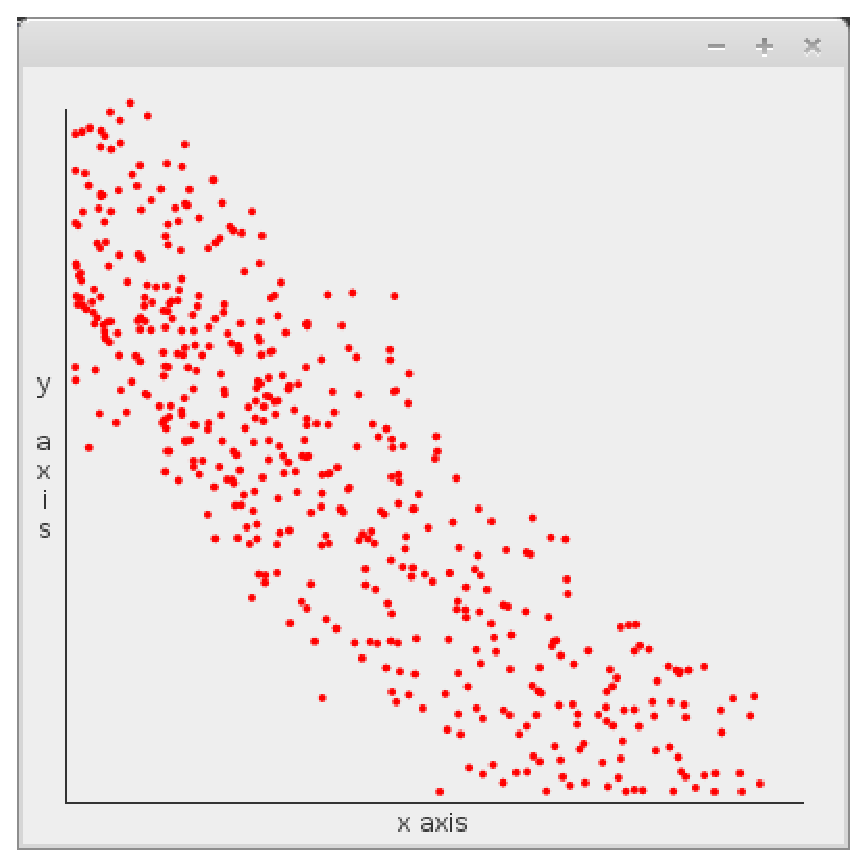
\includegraphics[width=0.24\textwidth]{figs/anti.eps}}
    \hspace{0.01em}
  \subfigbottomskip = 2pt  \subfigure[Correlated Distribution]
    {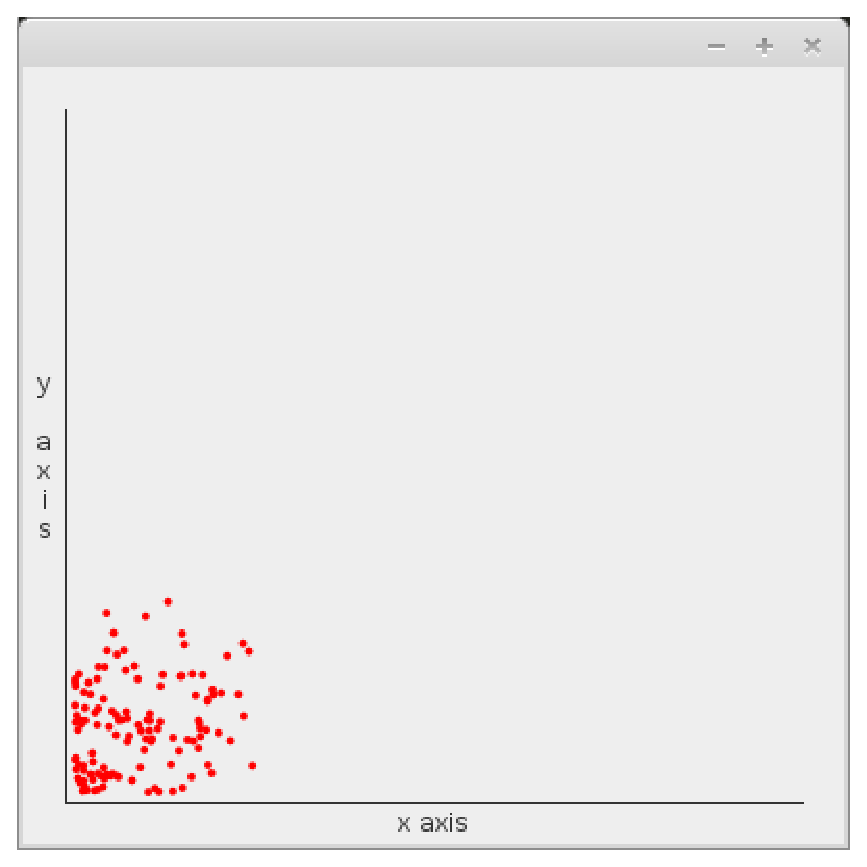
\includegraphics[width=0.24\textwidth]{figs/corr.eps}}

    \caption{Data Point Distribution after phase 1.}
    \label{fig:shape}
    \end{center}
\vspace{-10pt}
\end{figure*}

An experiment id conducted to depict the shape of instance distribution. The detailed experiment environment is illustrated as follows. In the two-dimensional space, objects are distributed between [0, 1] in domain of each dimension. Three varieties of object distribution (independent distribution, correlated distribution, and anti-correlated distribution) are tested respectively. The cardinality of objects is 5000. For each object, instances are created under a rectangle region, the edge size of which follows a normal distribution in range [0, 0.2] with expectation 0.1 and standard deviation 0.025.
The number of instances in each object follows uniform distribution in range [1, 100, and the first quadrant is evenly splitted into 6 angles. We apply the pruning algorithm in the first phase, filter objects which could not be in the $p$-skyline set. After that, we collected the objects which are still remained in each region, and paint all of them in the x-y axis. Figure~\ref{fig:shape} showed the result. For Independent or Anti-correlated data, many instances are remained. Therefore, the Strategy proposed in the merging phase should be able to apply for any variety of data distribution, especially for Independent and Anti-correlated data.

\subsection{Rectangle Splitting}
\begin{figure}[t]
\vspace{-15pt}
\centering
  \centerline{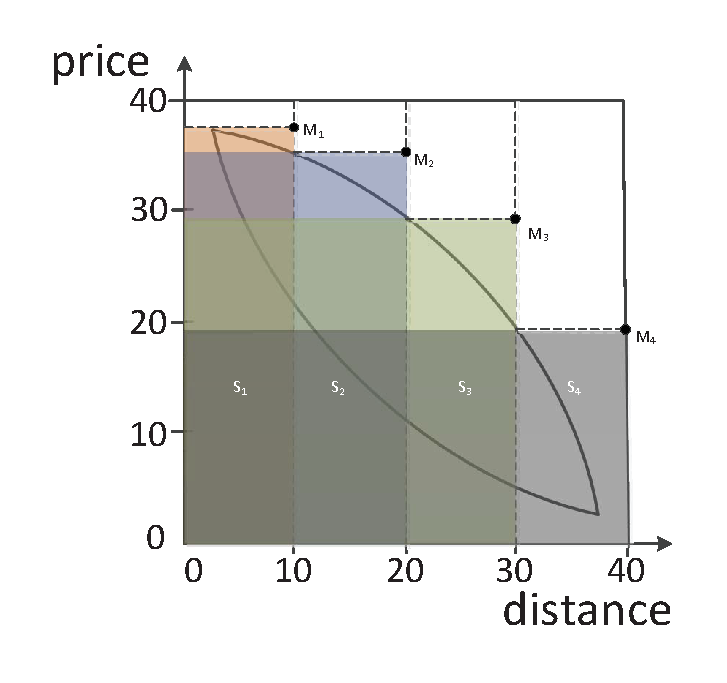
\psfig{file=figs/grid-merge.eps,width=4.0in}}
  \caption{Merging Phase}
  \vspace{-15pt}
  \label{figure:gridMerge}
\end{figure}

In this section, we propose an approach to efficiently evaluate skyline probability for  remained candidate objects. To utilize the MapReduce framework, we partition remained data to several domains which are able to work individually. The intuitive is to split data into several partitions, and each partition is not affected by others. Take Figure~\ref{figure:gridMerge} as an example. Data is distributed like spindle shape. Rectangles of different colors are drawn and any instance is covered by at least one rectangle. Data covered by a rectangle is sent to separate machine. It is found that object candidates in a machine are only dominated by instances in this rectangle, and skyline probability is easily computed.


Assume the remained instances are form the anti-correlated distribution (See Figure~\ref{figure:gridMerge}). The whole space is split into 4 parts $S_1, S_2, \dots, S_4$ based on X axis evenly partitioned. The maximum coordinate points (maximum coordinate in every dimension) is collected for each partition. Each maximum coordinate point denoted by $M_i$, is dominated by any instance in $S_i$. Then each grid region is rounded by the origin and the maximum point. In Figure~\ref{figure:gridMerge}, green area represents only instances which dominate the instances in $S_3$. Therefore, for computing instance skyline probability in $S_3$, it only needs instances in green area.

Recall that we have two remained sets of data $C_o$ and $I$. To avoid repeatedly computing, we propose a dynamic mapping strategy to send data to separate reducer evenly.



Followed by the example, the data is partitioned based on evenly along the x-axis. Given the the number of reducers $n$, the data is partitioned into n parts. Meanwhile, mapping method groups data into $N$ groups. Every group has two types of data, instances in $C_o$ and $I$ respectively. Take Figure~\ref{figure:gridMerge} as an example. The instances of $C_o$ in $S_2$ is in $S_2$ rectangle, and instances in the blue area are instance set $I$, which dominates $C_o$. Based on the grouping scheme, the mapping phase maps the two types of data to every slave machine. It is obvious that the choice of $n$ affects the efficiency of skyline probability computing. In the experiment section, we observe the performance trend with the variety of $n$.

In the reduce phase, skyline probability of every instance is computed. Assume an instance $p$ is in a partition $V^A$. Since $p$ is only dominated by corresponding region of instances, the instance skyline probability $SkyProb(p)$ is obtained using the standard approach. It finds all instances which instance $p$ by iterating all instances in this partition, and do Equations introduced in the Section~\ref{sec:prelim}. Then instance skyline probability of every instance is exported to a file in each partition.

After every instance in $C_o$ obtains its instance skyline probability, the second phase is completed. object skyline probability is grouped by iterating all instance skyline probability by Equation~\ref{equ_final}. $p-$skyline objects area able to be obtained by retrieving objects whose object skyline probability is larger than or equal to $p$.



\section{Experimental Validation}\label{sec:expr}
\begin{table}[t]
\begin{center}
    \begin{tabular}{|c|p{2cm}|}
    \hline
    Parameters & Default Values\\ \hline
    \hline
    $d$ (dimensions) & 3 \\ \hline
    $t$ (No. of machines) & 10 \\ \hline
    $|O|$ (object number) & $10^4$ \\ \hline
    $|P|$ (No. of pivot points in $P$) & 5 \\  \hline
    $l$ (No. partitions in Second Phase) & 5 \\   \hline
    \end{tabular}
\end{center}
\vspace{-8pt} \caption{Experimental parameter values.}
\label{tab_para} \vspace{-8pt}
\end{table}

In this section, we first evaluate our proposed Rectangle pruning methods on a single node. Then, we implemented our MapReduce Distributed System using Akka for communication between nodes. The introduction of MapReduce framework
For fair comparison, we developed a single MapReduce phase solution as a baseline solution. All solutions were implemented in Java and Scala.

The experiments were conducted on a 24-node shared-nothing
cluster. Each node was equipped with one Intel Xeon 2.4 GHz
processor, 2 GBytes of memory. All nodes were connected by GigaBit
Ethernet network. We utilized the default configuration in Hadoop.
Uniform, correlated and anti-related datasets were randomly generated in a
five-dimensional space. The parallel solutions were executed with
eight nodes by default. Simulation results were recorded after the
system model reached a steady state.


\subsection{Experimental Evaluation}
To compare the performance between three-phase, two-phase Hadoop implementations in one cluster and the straightforward implementation on a single machine, we implemented the three algorithms and conducted a experimental evaluation.

There're several observations found in the experiment:


1). Let me first introduce the result of single-machine algorithm. With increasing size of the dataset, the computing time is increasing exponentially. And the most arduous part in the whole computing procedure is in Equation2.

In the first experiment set, we randomly generated 100 objects, and 1 thousand instances per object. The whole computing procedure for Equation2 involves computing the local skyline probability between any pair of two objects. That is 215.6 seconds in our result. In addition, it needs 0.2s for Equation3 process and 0.02s for Equation4 process. Therefore, the whole running time is less than 216s. It can be found that 99\% of the time lies on Equation2. However, in our hadoop implementation, the whole query time is about 15 mins. Therefore, if the dataset is small, the time consumed in Hadoop is less than one in single-machine algorithm.

In the second experiment set, we randomly generated 100 objects, and 10 thousand instances per object. The test shows that it needs 5 seconds to run Equation2 for every pair of objects. Since we have \(C_{100}^{2}\) pairs, and the time in all is estimated to be more than 7 hours. However, the time consumed in the hadoop implementation is about 4 hours.

2). When compared between two Hadoop implementations, the two-phase Mapreduce framework is always faster than three-phase one. The reason is that the amount of computing is little in the third phase of the three-phase framework, and merging the second and third phase into one phase reduces one copy of reading data from the HDFS to memory, increasing I/O efficiency.

\subsection{Summary}
EX (Exhaustive) is an exhaustive algorithm for computing skyline probability in parallel environment. Our approach use two optimized way to speed up the skyline probability computation: one is Rectangle optimization in the first MapReduce phase, the other is one in the second phase.

\begin{itemize}
\item vary the object number

\item vary $p$

\item vary dimension

\item how much percent of data is able to be pruned by the first and third pruning rules provided, given the number of partitions, and the number of pivot points. Meanwhile, the response time is measured.

\item Given the number of partitions in the Second MapReduce phase, the response time of the reduce phase is measured.

\item all evaluation has three types of data distribution: Correlated, anti-correlated, independent.

\item communication cost

\end{itemize}



\begin{table*}[t]
%\vspace*{-15pt}
  \centering
\makeatletter
    \long\def\@makecaption#1#2{%
        \vskip\abovecaptionskip
        \centering
        #1 #2\par
        \vskip\belowcaptionskip}
\makeatother
  \caption{6 partitions}
    \vspace*{3pt}
  \footnotesize

  \label{table:partition6}
  \begin{tabular}{|c||c|c|c|c|c|c|c|c|c|}
  \hline
  \multirow{2}{*}{Partition} &  \multicolumn{3}{|c|}{iD2T2M0C5000} & \multicolumn{3}{|c|}{cD2T2M0C5000} &\multicolumn{3}{|c|}{aD2T2M0C5000} \\\cline{2-10}
    &  original No. & after Prune1 & after Prune3 & original No. & after Prune1 & after Prune3 & original No. & after Prune1 & after Prune3\\\hline\hline

\cline{2-10}
    1 &  734 & 72 & 43 & 354 & 202 & 35 & 1050  & 532 & 78 \\\hline

\cline{2-10}
    2 &  893 & 13 & 11 & 1225 & 290 & 15 & 1526 & 663 & 25 \\\hline

\cline{2-10}
    3 &  1171 & 7 & 5 & 3522 & 347 & 22 & 1651 & 692 & 24 \\\hline
    
\cline{2-10}
    4 &  1175 & 8 & 7 & 3587 & 319& 12 & 1644 & 842 & 34 \\\hline

\cline{2-10}
    5 &  873 & 20 & 11 & 1321 & 257 & 11 & 1605 & 916 & 37 \\\hline

\cline{2-10}
    6 &  717 & 84 & 36 & 379 & 106 & 13 & 1154 & 427 & 69 \\\hline

  \end{tabular}
  \vspace*{-17pt}
\end{table*}


\begin{table*}[t]
%\vspace*{-15pt}
  \centering
\makeatletter
    \long\def\@makecaption#1#2{%
        \vskip\abovecaptionskip
        \centering
        #1 #2\par
        \vskip\belowcaptionskip}
\makeatother
  \caption{4 partitions}
    \vspace*{3pt}
  \footnotesize

  \label{table:partition4}
  \begin{tabular}{|c||c|c|c|c|c|c|c|c|c|}
  \hline
  \multirow{2}{*}{Partition} &  \multicolumn{3}{|c|}{iD2T2M0C5000} & \multicolumn{3}{|c|}{cD2T2M0C5000} &\multicolumn{3}{|c|}{aD2T2M0C5000} \\\cline{2-10}
    &  original No. & after Prune1 & after Prune3 & original No. & after Prune1 & after Prune3 & original No. & after Prune1 & after Prune3\\\hline\hline

\cline{2-10}
    1 &  1101 & 72 & 41 & 726 & 268 & 35 & 1480 & 519 & 85 \\\hline

\cline{2-10}
    2 &  1563 & 8 & 8 & 3689 & 383 & 23 & 2027 & 818 & 39 \\\hline

\cline{2-10}
    3 &  1583 & 9 & 7 & 3766 & 357 & 12 & 2083 & 967 & 54 \\\hline
    
\cline{2-10}
    4 &  1089 & 69 & 38 & 753 & 137 & 15 & 1622 & 549 & 88 \\\hline
    
  \end{tabular}
  \vspace*{-17pt}
\end{table*}


\begin{table*}[t]
%\vspace*{-15pt}
  \centering
\makeatletter
    \long\def\@makecaption#1#2{%
        \vskip\abovecaptionskip
        \centering
        #1 #2\par
        \vskip\belowcaptionskip}
\makeatother
  \caption{2 partitions}
    \vspace*{3pt}
  \footnotesize

  \label{table:partition4}
  \begin{tabular}{|c||c|c|c|c|c|c|c|c|c|}
  \hline
  \multirow{2}{*}{Partition} &  \multicolumn{3}{|c|}{iD2T2M0C5000} & \multicolumn{3}{|c|}{cD2T2M0C5000} &\multicolumn{3}{|c|}{aD2T2M0C5000} \\\cline{2-10}
    &  original No. & after Prune1 & after Prune3 & original No. & after Prune1 & after Prune3 & original No. & after Prune1 & after Prune3\\\hline\hline

\cline{2-10}
    1 &  2577 & 73 & 38 & 3762 & 398 & 44 & 2834 & 842 & 112 \\\hline

\cline{2-10}
    2 &  2511 & 72 & 38 & 3844 & 221 & 22 & 2964 & 957 & 131 \\\hline
    
  \end{tabular}
  \vspace*{-17pt}
\end{table*}



\begin{table*}[t]
%\vspace*{-15pt}
  \centering
\makeatletter
    \long\def\@makecaption#1#2{%
        \vskip\abovecaptionskip
        \centering
        #1 #2\par
        \vskip\belowcaptionskip}
\makeatother
  \caption{6 partitions in Three Dimension}
    \vspace*{3pt}
  \footnotesize

  \label{table:partition6inThree}
  \begin{tabular}{|c||c|c|c|c|c|c|c|c|c|}
  \hline
  \multirow{2}{*}{Partition} &  \multicolumn{3}{|c|}{iD2T2M0C5000} & \multicolumn{3}{|c|}{cD2T2M0C5000} &\multicolumn{3}{|c|}{aD2T2M0C5000} \\\cline{2-10}
    &  original No. & after Prune1 & after Prune3 & original No. & after Prune1 & after Prune3 & original No. & after Prune1 & after Prune3\\\hline\hline

\cline{2-10}
    1 &  1106 & 17 & 10 & 1066 & 187 & 146 & 1126  & 19 & 9 \\\hline

\cline{2-10}
    2 &  1149 & 14 & 10 & 387 & 57 & 40 & 1152 & 14 & 12 \\\hline

\cline{2-10}
    3 &  750 & 13 & 8 & 1171 & 234 & 186 & 748 & 15 & 11 \\\hline
    
\cline{2-10}
    4 &  1132 & 12 & 2 & 1092 & 180& 155 & 1131 & 16 & 4 \\\hline
    
\cline{2-10}
    5 &  1266 & 14 & 13 & 367 & 57 & 37 & 1255 & 14 & 8 \\\hline
    
\cline{2-10}
    6 &  789 & 13 & 14 & 1267 & 212 & 179 & 788 & 15 & 10 \\\hline

  \end{tabular}
  \vspace*{-17pt}
\end{table*}


\begin{table*}[t]
%\vspace*{-15pt}
  \centering
\makeatletter
    \long\def\@makecaption#1#2{%
        \vskip\abovecaptionskip
        \centering
        #1 #2\par
        \vskip\belowcaptionskip}
\makeatother
  \caption{4 partitions in Three Dimension}
    \vspace*{3pt}
  \footnotesize

  \label{table:partition4inThree}
  \begin{tabular}{|c||c|c|c|c|c|c|c|c|c|}
  \hline
  \multirow{2}{*}{Partition} &  \multicolumn{3}{|c|}{iD2T2M0C5000} & \multicolumn{3}{|c|}{cD2T2M0C5000} &\multicolumn{3}{|c|}{aD2T2M0C5000} \\\cline{2-10}
    &  original No. & after Prune1 & after Prune3 & original No. & after Prune1 & after Prune3 & original No. & after Prune1 & after Prune3\\\hline\hline

\cline{2-10}
    1 &  1413 & 61 & 44 & 1392 & 211 & 171 & 2081 & 6 & 5 \\\hline

\cline{2-10}
    2 &  1159 & 66 & 37 & 1171 & 223 & 185 & 748 & 5 & 5 \\\hline

\cline{2-10}
    3 &  1447 & 63 & 35 & 1399 & 194 & 160 & 2176 & 9 & 8 \\\hline
    
\cline{2-10}
    4 &  1228 & 92 & 46 & 1267 & 202 & 173 & 788 & 8 & 7 \\\hline
    
  \end{tabular}
  \vspace*{-17pt}
\end{table*}


\begin{table*}[t]
%\vspace*{-15pt}
  \centering
\makeatletter
    \long\def\@makecaption#1#2{%
        \vskip\abovecaptionskip
        \centering
        #1 #2\par
        \vskip\belowcaptionskip}
\makeatother
  \caption{2 partitions in Three Dimension}
    \vspace*{3pt}
  \footnotesize

  \label{table:partition4InThree}
  \begin{tabular}{|c||c|c|c|c|c|c|c|c|c|}
  \hline
  \multirow{2}{*}{Partition} &  \multicolumn{3}{|c|}{iD2T2M0C5000} & \multicolumn{3}{|c|}{cD2T2M0C5000} &\multicolumn{3}{|c|}{aD2T2M0C5000} \\\cline{2-10}
    &  original No. & after Prune1 & after Prune3 & original No. & after Prune1 & after Prune3 & original No. & after Prune1 & after Prune3\\\hline\hline

\cline{2-10}
    1 &  2523 & 116 & 83 & 2505 & 428 & 348 & 2670 & 26 & 7 \\\hline

\cline{2-10}
    2 &  2603 & 149 & 84 & 2608 & 387 & 333 & 2792 & 16 & 6 \\\hline
    
  \end{tabular}
  \vspace*{-17pt}
\end{table*}



\vspace*{50pt}
\begin{table*}[t]
%\vspace*{-15pt}
  \centering
\makeatletter
    \long\def\@makecaption#1#2{%
        \vskip\abovecaptionskip
        \centering
        #1 #2\par
        \vskip\belowcaptionskip}
\makeatother
  \caption{6 partitions}
    \vspace*{3pt}
  \footnotesize

  \label{table:partition6}
  \begin{tabular}{|c||c|c|c|c|c|c|c|c|c|}
  \hline
  \multirow{2}{*}{Partition} &  \multicolumn{3}{|c|}{iD2T2M0C5000} & \multicolumn{3}{|c|}{cD2T2M0C5000} &\multicolumn{3}{|c|}{aD2T2M0C5000} \\\cline{2-10}
    &  naive(ms) & prune1-2(ms) & prune1-2-3(ms) & naive(ms) & prune1-2(ms) & prune1-2-3(ms) & naive(ms) & prune1-2(ms) & prune1-2-3(ms) \\\hline \hline

\cline{2-10}
    1 &  4064 & 210 & 835 & 178 & 130 & 602 & 2213  & 532 & 1520 \\\hline

\cline{2-10}
    2 &  5200 & 18 & 205 & 1001 & 179 & 423 & 2322 & 532 & 1038 \\\hline

\cline{2-10}
    3 &  9732 & 6 & 203 & 10955 &  458 & 817 & 2629 & 579 & 1069 \\\hline
    
\cline{2-10}
    4 &  9426 & 6 & 123 & 11306 &  441& 655 & 2448 & 700 & 1347 \\\hline
    
\cline{2-10}
    5 &  5371 & 7 & 117 & 884 &  136 & 298 & 2453 & 732 & 1527 \\\hline
    
\cline{2-10}
    6 &  3753 & 114 & 302 & 51 & 15 & 149 & 1805 & 276 & 689 \\\hline

  \end{tabular}
  \vspace*{-17pt}
\end{table*}


\begin{table*}[t]
%\vspace*{-15pt}
  \centering
\makeatletter
    \long\def\@makecaption#1#2{%
        \vskip\abovecaptionskip
        \centering
        #1 #2\par
        \vskip\belowcaptionskip}
\makeatother
  \caption{4 partitions}
    \vspace*{3pt}
  \footnotesize

  \label{table:partition4}
  \begin{tabular}{|c||c|c|c|c|c|c|c|c|c|}
  \hline
  \multirow{2}{*}{Partition} &  \multicolumn{3}{|c|}{iD2T2M0C5000} & \multicolumn{3}{|c|}{cD2T2M0C5000} &\multicolumn{3}{|c|}{aD2T2M0C5000} \\\cline{2-10}
    &  naive(ms) & prune1-2(ms) & prune1-2-3(ms) & naive(ms) & prune1-2(ms) & prune1-2-3(ms) & naive(ms) & prune1-2(ms) & prune1-2-3(ms) \\\hline \hline

\cline{2-10}
    1 &  9077 & 240 & 947 & 482 & 177 & 795 & 4103 & 771 & 2035 \\\hline

\cline{2-10}
    2 &  17444 & 18 & 186 & 15771 & 609 & 984 & 5146 & 926 & 1667 \\\hline

\cline{2-10}
    3 &  17874 & 9 & 204 & 16606 & 543 & 785 & 5027 & 1137 & 2201 \\\hline
    
\cline{2-10}
    4 &  8952 & 145 & 330 & 271 & 42 & 157 & 4358 & 618 & 1243 \\\hline
    
  \end{tabular}
  \vspace*{-17pt}
\end{table*}


\begin{table*}[t]
%\vspace*{-15pt}
  \centering
\makeatletter
    \long\def\@makecaption#1#2{%
        \vskip\abovecaptionskip
        \centering
        #1 #2\par
        \vskip\belowcaptionskip}
\makeatother
  \caption{2 partitions}
    \vspace*{3pt}
  \footnotesize

  \label{table:partition4}
  \begin{tabular}{|c||c|c|c|c|c|c|c|c|c|}
  \hline
  \multirow{2}{*}{Partition} &  \multicolumn{3}{|c|}{iD2T2M0C5000} & \multicolumn{3}{|c|}{cD2T2M0C5000} &\multicolumn{3}{|c|}{aD2T2M0C5000} \\\cline{2-10}
    &  naive(ms) & prune1-2(ms) & prune1-2-3(ms) & naive(ms) & prune1-2(ms) & prune1-2-3(ms) & naive(ms) & prune1-2(ms) & prune1-2-3(ms) \\\hline \hline

\cline{2-10}
    1 &  51631 & 353 & 1158 & 16783 & 841 & 1735 & 20143 & 1882 & 4041 \\\hline

\cline{2-10}
    2 &  52009 & 268 & 554 & 18263 & 435 & 643 & 20859 & 2085 & 4363 \\\hline
    
  \end{tabular}
  \vspace*{-17pt}
\end{table*}



\begin{table*}[t]
%\vspace*{-15pt}
  \centering
\makeatletter
    \long\def\@makecaption#1#2{%
        \vskip\abovecaptionskip
        \centering
        #1 #2\par
        \vskip\belowcaptionskip}
\makeatother
  \caption{6 partitions in Three Dimension}
    \vspace*{3pt}
  \footnotesize

  \label{table:partition6inThree}
  \begin{tabular}{|c||c|c|c|c|c|c|c|c|c|}
  \hline
  \multirow{2}{*}{Partition} &  \multicolumn{3}{|c|}{iD2T2M0C5000} & \multicolumn{3}{|c|}{cD2T2M0C5000} &\multicolumn{3}{|c|}{aD2T2M0C5000} \\\cline{2-10}
    &  naive(ms) & prune1-2(ms) & prune1-2-3(ms) & naive(ms) & prune1-2(ms) & prune1-2-3(ms) & naive(ms) & prune1-2(ms) & prune1-2-3(ms) \\\hline \hline

\cline{2-10}
    1 &  5663 & 203 & 921 & 2243 & 72 & 665 & 6247  & 318 & 1265 \\\hline

\cline{2-10}
    2 &  10115 & 46 & 267 & 47671 & 47 & 347 & 9552 & 222 & 623 \\\hline

\cline{2-10}
    3 &  4732 & 50 & 297 & 112 & 5 & 178 & 5062 & 163 & 508 \\\hline
    
\cline{2-10}
    4 &  4875 & 79 & 262 & 1165 & 9 & 123 & 6395 & 187 & 488 \\\hline
    
\cline{2-10}
    5 &  11461 & 81 & 236 & 55666 & 22 & 235 & 10420 & 215 & 449 \\\hline
    
\cline{2-10}
    6 &  5804 & 110 & 296 & 158 & 2 & 94 & 5415 & 169 & 493 \\\hline

  \end{tabular}
  \vspace*{-17pt}
\end{table*}


\begin{table*}[t]
%\vspace*{-15pt}
  \centering
\makeatletter
    \long\def\@makecaption#1#2{%
        \vskip\abovecaptionskip
        \centering
        #1 #2\par
        \vskip\belowcaptionskip}
\makeatother
  \caption{4 partitions in Three Dimension}
    \vspace*{3pt}
  \footnotesize

  \label{table:partition4inThree}
  \begin{tabular}{|c||c|c|c|c|c|c|c|c|c|}
  \hline
  \multirow{2}{*}{Partition} &  \multicolumn{3}{|c|}{iD2T2M0C5000} & \multicolumn{3}{|c|}{cD2T2M0C5000} &\multicolumn{3}{|c|}{aD2T2M0C5000} \\\cline{2-10}
    &  naive(ms) & prune1-2(ms) & prune1-2-3(ms) & naive(ms) & prune1-2(ms) & prune1-2-3(ms) & naive(ms) & prune1-2(ms) & prune1-2-3(ms) \\\hline \hline

\cline{2-10}
    1 &  18532 & 257 & 998 & 32354 & 103 & 780 & 16427 & 596 & 1643 \\\hline

\cline{2-10}
    2 &  11271 & 127 & 324 & 3585 & 17 & 1647 & 10852 & 347 & 878 \\\hline

\cline{2-10}
    3 &  18049 & 123 & 352 & 34568 & 25 & 236 & 16147 & 377 & 904 \\\hline
    
\cline{2-10}
    4 &  13742 & 186 & 397 & 4043 & 6 & 120 & 12966 & 347 & 900 \\\hline
    
  \end{tabular}
  \vspace*{-17pt}
\end{table*}


\begin{table*}[t]
%\vspace*{-15pt}
  \centering
\makeatletter
    \long\def\@makecaption#1#2{%
        \vskip\abovecaptionskip
        \centering
        #1 #2\par
        \vskip\belowcaptionskip}
\makeatother
  \caption{2 partitions in Three Dimension}
    \vspace*{3pt}
  \footnotesize

  \label{table:partition4InThree}
  \begin{tabular}{|c||c|c|c|c|c|c|c|c|c|}
  \hline
  \multirow{2}{*}{Partition} &  \multicolumn{3}{|c|}{iD2T2M0C5000} & \multicolumn{3}{|c|}{cD2T2M0C5000} &\multicolumn{3}{|c|}{aD2T2M0C5000} \\\cline{2-10}
    &  naive(ms) & prune1-2(ms) & prune1-2-3(ms) & naive(ms) & prune1-2(ms) & prune1-2-3(ms) & naive(ms) & prune1-2(ms) & prune1-2-3(ms) \\\hline \hline

\cline{2-10}
    1 &  58577 & 536 & 1440 & 58079 & 163 & 862 & 55168 & 1584 & 3968 \\\hline

\cline{2-10}
    2 &  64964 & 710 & 1158 & 64775 & 69 & 301 & 60498 & 1448 & 3064 \\\hline
    
  \end{tabular}
  \vspace*{-17pt}
\end{table*}


% \begin{table*}
% \centering
% \makeatletter
%     \long\def\@makecaption#1#2{%
%         \vskip\abovecaptionskip
%         \centering
%         #1 #2\par
%         \vskip\belowcaptionskip}
% \makeatother
%   \caption{4 partitions with 5K |O| in MapReduce}
%     \vspace*{3pt}
%   \footnotesize

%   \label{table:asdf}
%   \begin{tabular}{|c||c|c|c|c|c|c|}
%   \hline
%   \multirow{2}{*}{Partition} &  \multicolumn{2}{|c|}{cD2T2M0C5000} & \multicolumn{2}{|c|}{iD2T2M0C5000} &\multicolumn{2}{|c|}{aD2T2M0C5000} \\\cline{2-7}
%     &  Map & Reduce & Map & Reduce & Map & Reduce \\\hline\hline

% \cline{2-7}
%     1 &  3k & 6k & 3k & 12k & 3k & 19k \\\hline

% \cline{2-7}
%     2 &  3k & 12k & 3k & 13k & 3k & 21k \\\hline

% \cline{2-7}
%     3 &  3k & 20k & 3k & 13k & 3k & 31k  \\\hline

% \cline{2-7}
%     4 &  3k & 20k & 3k & 14k & 3k & 32k  \\\hline

% \cline{2-7}
%     5 &  3k & 12k & 3k & 12k & 3k & 23k  \\\hline

% \cline{2-7}
%     6 &  3k & 6k & 3k & 11k & 3k & 19k  \\\hline

%   \end{tabular}
%   \vspace*{-17pt}
% \end{table*}




\begin{table*}[t]
%\vspace*{-15pt}
  \centering
\makeatletter
    \long\def\@makecaption#1#2{%
        \vskip\abovecaptionskip
        \centering
        #1 #2\par
        \vskip\belowcaptionskip}
\makeatother
  \caption{6 partitions with 50K |O|}
    \vspace*{3pt}
  \footnotesize

  \label{table:partition6}
  \begin{tabular}{|c||c|c|c|c|c|c|c|c|c|}
  \hline
  \multirow{2}{*}{Partition} &  \multicolumn{3}{|c|}{cD2T2M0C50000} & \multicolumn{3}{|c|}{iD2T2M0C50000} &\multicolumn{3}{|c|}{aD2T2M0C50000} \\\cline{2-10}
    &  original No. & after Prune1 & after Prune3 & original No. & after Prune1 & after Prune3 & original No. & after Prune1 & after Prune3\\\hline\hline

\cline{2-10}
    1 &  292 & 28 & 13 & 7213 & 384 & 65 & 7808  & 322 & 77 \\\hline

\cline{2-10}
    2 &  4741 & 56 & 18 & 8835 & 81 & 21 & 9257 & 39 & 17 \\\hline

\cline{2-10}
    3 &  24034 & 56 & 19 & 11722 & 41 & 10 & 9917 & 35 & 20 \\\hline
    
\cline{2-10}
    4 &  23902 & 72 & 17 & 11873 & 45 & 19 & 9913 & 42 & 14 \\\hline

\cline{2-10}
    5 &  4881 & 52 & 12 & 8886 & 77 & 15 & 9500 & 58 & 22 \\\hline

\cline{2-10}
    6 &  322 & 39 & 15 & 7073 & 189 & 70 & 8001 & 321 & 48 \\\hline

  \end{tabular}
  \vspace*{-17pt}
\end{table*}


\begin{table*}[t]
%\vspace*{-15pt}
  \centering
\makeatletter
    \long\def\@makecaption#1#2{%
        \vskip\abovecaptionskip
        \centering
        #1 #2\par
        \vskip\belowcaptionskip}
\makeatother
  \caption{4 partitions with 50K |O|}
    \vspace*{3pt}
  \footnotesize

  \label{table:partition4}
  \begin{tabular}{|c||c|c|c|c|c|c|c|c|c|}
  \hline
  \multirow{2}{*}{Partition} &  \multicolumn{3}{|c|}{cD2T2M0C50000} & \multicolumn{3}{|c|}{iD2T2M0C50000} &\multicolumn{3}{|c|}{aD2T2M0C50000} \\\cline{2-10}
    &  original No. & after Prune1 & after Prune3 & original No. & after Prune1 & after Prune3 & original No. & after Prune1 & after Prune3\\\hline\hline

\cline{2-10}
    1 &  1486 & 33 & 17 & 10956 & 389 & 66 & 12029 & 331 & 83 \\\hline

\cline{2-10}
    2 &  26485 & 59 & 23 & 15784 & 49 & 13 & 14127 & 37 & 27 \\\hline

\cline{2-10}
    3 &  26480 & 68 & 18 & 15974 & 63 & 18 & 14191 & 65 & 27 \\\hline
    
\cline{2-10}
    4 &  1538 & 52 & 17 & 10878 & 194 & 69 & 12394 & 325 & 51 \\\hline
    
  \end{tabular}
  \vspace*{-17pt}
\end{table*}



\clearpage

\vspace*{50pt}
\begin{table*}[t]
%\vspace*{-15pt}
  \centering
\makeatletter
    \long\def\@makecaption#1#2{%
        \vskip\abovecaptionskip
        \centering
        #1 #2\par
        \vskip\belowcaptionskip}
\makeatother
  \caption{6 partitions (Time: us)}
    \vspace*{3pt}
  \footnotesize

  \label{table:partition6}
  \begin{tabular}{|c||c|c|c|c|c|c|c|c|c|}
  \hline
  \multirow{2}{*}{Partition} &  \multicolumn{3}{|c|}{cD2T2M0C50000} & \multicolumn{3}{|c|}{iD2T2M0C50000} &\multicolumn{3}{|c|}{aD2T2M0C50000} \\\cline{2-10}
    &  naive(ms) & prune1-2(ms) & prune1-2-3(ms) & naive(ms) & prune1-2(ms) & prune1-2-3(ms) & naive(ms) & prune1-2(ms) & prune1-2-3(ms) \\\hline \hline

\cline{2-10}
    1 &  666 & 81 & 1307 & 354417 & 3752 & 7206 & 445281  & 3570 & 6284 \\\hline

\cline{2-10}
    2 &  139598 & 152 & 1295 & 461749 & 506 & 1711 & 565292 & 550 & 1671 \\\hline

\cline{2-10}
    3 &  4038701 & 1231 & 2915 & 845655 & 247 & 1450 & 632030 & 649 & 1702 \\\hline
    
\cline{2-10}
    4 &  3936687 & 1327 & 2761 & 883083 & 358 & 1555 & 643929 & 597 & 1643 \\\hline
    
\cline{2-10}
    5 &  143735 & 124 & 1049 & 48208 &  428 & 1553 & 627326 & 748 & 1828 \\\hline
    
\cline{2-10}
    6 &  484 & 60 & 825 & 338058 & 2196 & 3549 & 450133 & 4001 & 6177 \\\hline

  \end{tabular}
  \vspace*{-17pt}
\end{table*}




\begin{table*}[t]
%\vspace*{-15pt}
  \centering
\makeatletter
    \long\def\@makecaption#1#2{%
        \vskip\abovecaptionskip
        \centering
        #1 #2\par
        \vskip\belowcaptionskip}
\makeatother
  \caption{4 partitions (Time: us)}
    \vspace*{3pt}
  \footnotesize

  \label{table:partition4}
  \begin{tabular}{|c||c|c|c|c|c|c|c|c|c|}
  \hline
  \multirow{2}{*}{Partition} &  \multicolumn{3}{|c|}{cD2T2M0C5000} & \multicolumn{3}{|c|}{iD2T2M0C5000} &\multicolumn{3}{|c|}{aD2T2M0C5000} \\\cline{2-10}
    &  naive(ms) & prune1-2(ms) & prune1-2-3(ms) & naive(ms) & prune1-2(ms) & prune1-2-3(ms) & naive(ms) & prune1-2(ms) & prune1-2-3(ms) \\\hline \hline

\cline{2-10}
    1 &  11369 & 119 & 1536 & 844773 & 5721 & 8986 & 1045580 & 5222 & 8040 \\\hline

\cline{2-10}
    2 &  4859706 & 1166 & 3207 & 1601874 & 667 & 1924 & 1367131 & 1266 & 2541 \\\hline

\cline{2-10}
    3 &  4806449 & 1230 & 3016 & 1660244 & 674 & 1895 & 1390984 & 1250 & 2475 \\\hline
    
\cline{2-10}
    4 &  11858 & 67 & 923 & 821776 & 3250 & 4662 & 1148428 & 6292 & 8563 \\\hline
    
  \end{tabular}
  \vspace*{-17pt}
\end{table*}




\begin{table*}[t]
%\vspace*{-15pt}
  \centering
\makeatletter
    \long\def\@makecaption#1#2{%
        \vskip\abovecaptionskip
        \centering
        #1 #2\par
        \vskip\belowcaptionskip}
\makeatother
  \caption{4 partitions with 5K |O| in MapReduce (Time: ms)}
    \vspace*{3pt}
  \footnotesize

  \label{table:partition6}
  \begin{tabular}{|c||c|c|c|c|c|c|}
  \hline
  \multirow{2}{*}{Partition} &  \multicolumn{2}{|c|}{cD2T2M0C50000} & \multicolumn{2}{|c|}{iD2T2M0C50000} &\multicolumn{2}{|c|}{aD2T2M0C50000} \\\cline{2-7}
    &  Map & Reduce & Map & Reduce & Map & Reduce \\\hline\hline

\cline{2-7}
    1 &  3k & 9k & 3k & 14k & 3k & 22k \\\hline

\cline{2-7}
    2 &  3k & 26k & 3k & 16k & 3k & 36k \\\hline

\cline{2-7}
    3 &  3k & 26k & 3k & 15k & 3k & 34k  \\\hline
    
\cline{2-7}
    4 &  3k & 9k & 3k & 14k & 3k & 24k  \\\hline

  \end{tabular}
  \vspace*{-17pt}
\end{table*}




\begin{table*}[t]
%\vspace*{-15pt}
  \centering
\makeatletter
    \long\def\@makecaption#1#2{%
        \vskip\abovecaptionskip
        \centering
        #1 #2\par
        \vskip\belowcaptionskip}
\makeatother
  \caption{6 partitions with 5K |O| in MapReduce (Time: ms)}
    \vspace*{3pt}
  \footnotesize

  \label{table:partition6}
  \begin{tabular}{|c||c|c|c|c|c|c|}
  \hline
  \multirow{2}{*}{Partition} &  \multicolumn{2}{|c|}{cD2T2M0C5000} & \multicolumn{2}{|c|}{iD2T2M0C5000} &\multicolumn{2}{|c|}{aD2T2M0C5000} \\\cline{2-7}
    &  Map & Reduce & Map & Reduce & Map & Reduce \\\hline\hline


\cline{2-7}
    1 &  3k & 6k & 3k & 12k & 3k & 19k \\\hline

\cline{2-7}
    2 &  3k & 12k & 3k & 13k & 3k & 21k \\\hline

\cline{2-7}
    3 &  3k & 20k & 3k & 13k & 3k & 31k  \\\hline

\cline{2-7}
    4 &  3k & 20k & 3k & 14k & 3k & 32k  \\\hline

\cline{2-7}
    5 &  3k & 12k & 3k & 12k & 3k & 23k  \\\hline

\cline{2-7}
    6 &  3k & 6k & 3k & 11k & 3k & 19k  \\\hline

  \end{tabular}
  \vspace*{-17pt}
\end{table*}




\begin{table*}[t]
%\vspace*{-15pt}
  \centering
\makeatletter
    \long\def\@makecaption#1#2{%
        \vskip\abovecaptionskip
        \centering
        #1 #2\par
        \vskip\belowcaptionskip}
\makeatother
  \caption{4 partitions with 50K |O| in MapReduce (Time: ms)}
    \vspace*{3pt}
  \footnotesize

  \label{table:partition6}
  \begin{tabular}{|c||c|c|c|c|c|c|}
  \hline
  \multirow{2}{*}{Partition} &  \multicolumn{2}{|c|}{cD2T2M0C50000} & \multicolumn{2}{|c|}{iD2T2M0C50000} &\multicolumn{2}{|c|}{aD2T2M0C50000} \\\cline{2-7}
    &  Map & Reduce & Map & Reduce & Map & Reduce \\\hline\hline

\cline{2-7}
    1 & 8k & 7k  & 8k & 907k & 8k & 2284k \\\hline

\cline{2-7}
    2 & 8k & 3835k  & 8k & 2107k & 8k & 2612k \\\hline

\cline{2-7}
    3 & 8k & 3889k  & 8k & 2045k & 8k & 2632k  \\\hline
    
\cline{2-7}
    4 & 8k & 7k  & 8k & 968k & 8k & 2325k  \\\hline

  \end{tabular}
  \vspace*{-17pt}
\end{table*}



\begin{table*}[t]
%\vspace*{-15pt}
  \centering
\makeatletter
    \long\def\@makecaption#1#2{%
        \vskip\abovecaptionskip
        \centering
        #1 #2\par
        \vskip\belowcaptionskip}
\makeatother
  \caption{6 partitions with 50K |O| in MapReduce (Time: ms)}
    \vspace*{3pt}
  \footnotesize

  \label{table:partition6}
  \begin{tabular}{|c||c|c|c|c|c|c|}
  \hline
  \multirow{2}{*}{Partition} &  \multicolumn{2}{|c|}{cD2T2M0C50000} & \multicolumn{2}{|c|}{iD2T2M0C50000} &\multicolumn{2}{|c|}{aD2T2M0C50000} \\\cline{2-7}
    &  Map & Reduce & Map & Reduce & Map & Reduce \\\hline\hline


\cline{2-7}
    1 &  8k & 6k & 8k & 801k & 8k & 2054k \\\hline

\cline{2-7}
    2 &  8k & 923k & 8k & 1749k & 8k & 2512k \\\hline

\cline{2-7}
    3 &  8k & 2634k & 8k & 1705k & 8k & 2512k  \\\hline

\cline{2-7}
    4 &  8k & 2988k & 8k & 1877k & 8k & 2606k  \\\hline

\cline{2-7}
    5 &  8k & 883k & 8k & 1793k & 8k & 2443k  \\\hline

\cline{2-7}
    6 &  8k & 6k & 8k & 786k & 8k & 1991k  \\\hline

  \end{tabular}
  \vspace*{-17pt}
\end{table*}

%\section{Conclusion}\label{sec:conc}
%\input{conc}


%\section*{Acknowledgements}
%\small
This research has been funded in part by the National Science
Foundation grants CNS-0831502 (CT) and CNS-0855251 (CRI).

%Any opinions, findings, and conclusions or recommendations
%expressed in this material are those of the author(s) and do not
%necessarily reflect the views of the National Science Foundation.


\small
\bibliographystyle{abbrv}
\bibliography{Ji_citations}

\end{document}
